\documentclass[reprint, nobibnotes, amssymb, amsmath, amsfonts, physics, mathtools, mathrsfs, floatfix]{revtex4-1}
\usepackage{graphicx}
\usepackage[english]{babel}

\newcommand{\redchi}{$\tilde{\chi}^2\,$}

\begin{document}

  \title{Relativistic Dispersion of Free Electrons}

  \author{Aman LaChapelle}
  \affiliation{The University of Chicago}

  \begin{abstract}
    We demonstrate the Hall Effect in a Germanium sample that is p-type doped with Gallium.  We observe hole conduction at low temperatures and measure a Hall coefficient of XXXXXXXX that has XXXXXXX correlation with temperature.  We measure an energy gap between valence and conduction bands in $Ge_{1-x}Ga_x$ of XXXX.
  \end{abstract}

  \maketitle
  \tableofcontents

  \section{Introduction and Theory}
    The Hall effect is an effect that occurs when we run a current through a region with a perpendicular magnetic field.  The classical picture is that the electrons which move in cyclotron orbits in the bulk will move in a skipping motion at the edge and create edge currents, significantly, a current that induces a voltage difference that is perpendicular to the applied current/voltage.  This effect was famously first noticed by Edwin Hall in 1879~\cite{classical_hall}.  Later on, after the formalism proposed by Landau and Lifschitz ~\cite{landau}, and the nearly concurrent discovery by Von Klitzing of the exact quantization of the Hall conductivity~\cite{Von_Klitzing} did the solid state physics community begin to understand the quantum effects behind the Hall effect.

    Shortly after the discovery of the Integer Quantum Hall Effect (IQHE), came the discovery of what is now called the Fractional Quantum Hall Effect (FQHE).  The first observation of the FQHE was by Horst St\"{o}rmer and Dan Tsui~\cite{stormer_tsui}, searching for the theorized Wigner crystal that would form from electrons in a solid under extremely high mangetic fields.  Just a year later Robert Laughlin introduced the Laughlin wave function that did an excellent job of explaining this effect - now understood to be because of fractional filling of the landau levels.

    Subsequent discoveries in the realm of quantum hall physics have mostly focused on topological nontriviality, and a current prevailing explanation uses Chern-Simons field theory to perform a singular gauge transformation in order to attach flux quanta to electrons in the form of vortices - a.k.a. zeros of the wave function.  We can think of the effect in a very simplistic way as electrons and vortices bound together in such a way that the electron wave function picks up a phase of $2\pi$ times the number of vortices that the electron is pinned to as it goes around.  This is (again very simplistically) an extension of the Aharonov-Bohm effect, and is beginning to be understood in terms of topological nontrivialities that are properties of the quantum system itself - another interpretation being the relation of the Berry phase to the Chern number of the system and characterizing its topological invariance.  It is important to recognize that much of this characterization occurs in real-space, which allows real-space measurements of system invariants such as the Chern number and other topological invariants.

    For our case, the classical theory provides enough formalism, as we are not dealing with a temperature, experimental resolution, or field at which partial filling factors come into play, we are only concerned with the voltage difference induced perpendicular to the induced voltage at a very classical level.  The essence of the Hall effect remains much the same - we will notice that the cause of the hall voltage is still due to the landau quantization (however at high filling factors/currents it is nearly continuous) and the edge states that arise as a result of this quantization.  We can, however, describe much of this formalism in the classical limit with Dr\"{u}de theory as follows.

    If we consider electrons/holes as simple masses traveling through a region with a certain net velocity (drift velocity) and time between scattering events (mean free time), where the current is described by
    \begin{equation}
      j = -nev_d
    \end{equation}
    we can then define a conductivity tensor and simply write down the Lorentz force equation to return the Hall Voltage and Resistance as the following:
    \begin{gather}
      R_H = \frac{1}{q n} = \frac{E_y}{j_x B_z} \label{hall_resist} \\
      V_H = R_H j_x B_z w \label{hall_volt}
    \end{gather}
    with $j_x$ the applied current and w the width of the sample.  It is important to note that we have defined the Hall Resistance in terms of the charge, $q$, when it is normally defined in terms of the electron charge, $-e$, or the hole charge, $+e$, depending on the primary charge carrier.

    Now, with a basic understanding of band theory, we can rewrite this a little in order to take better accounting of electrons and holes and potentially different scattering characteristics.  We rewrite the current (and the drift velocity) in terms of the mobility and get the following equations that allow us to take into account different charge carriers in different systems:
    \begin{gather}
      \mu_{h/e} = \frac{e \tau_e/h}{m_{e/h}^*} \label{mobility} \\
      \text{Which leads us to the following:} \nonumber \\
      \sigma = e(n_h\mu_h + n_e\mu_e) \label{conductivity} \\
      R_H = \frac{E_y}{j_x B_z} = \frac{\mu_h^2 n_h - \mu_e^2 n_e}{\sigma^2/e}
    \end{gather}
    with $\sigma$ being the conductivity we are familiar with from Ohm's law.  This formulation suggests the definition of a new quantity, the Hall mobility:
    \begin{equation}
      \mu_H = |R_H|\sigma \label{hall_mobility}
    \end{equation}
    which allows us to relate resistivity of a given semiconductor in and out of a magnetic field in a phenomenon known as magnetoresistance - which is the same phenomenon wherein we see peaks of resistivity at the quantized hall plateaus - the resistance in the induced direction increases sharply as we come to quantized values for the Hall resistance.

    There are two types of dopants for semiconductors - p-type and n-type.  n-type semiconductors donate negative charges, or electrons, to the semiconductor band structure, resulting in the main charge carrier being an electron that can move freely throughout the bulk.  P-type dopants accept electrons, creating holes in the band structure which still allows for charge flow but now holes are the dominant charge carrier.  This becomes manifestly true at low temperatures especially due to the fact that at low temperatures the electrons bound to the bulk atoms are stuck, and the only things moving will be the dopant particles (or quasiparticles as is the case with holes).

    \section{Experimental Methods}
    In order to measure the Hall voltage and from that the resistivity and the Hall coefficient, we made the following electrical measurements.  If we refer to Figure~\ref{circuit_diagram}, we notice that we run current through the sample in the direction from point 5 to point 6.  We can then directly measure the Hall voltage by measuring the difference between ports 1 and 2, or 3 and 4.  Now, it is possible that these ports are not perfectly horizontal with each other - that is, they might not be normal to both the current propagation \textbf{and} the magnetic field, and so we will take data by making rotations - henceforth referred to as '+' and '-'.  The idea is that if we take data at one orientation and then at the other, we will be able to simply average out the effect from the offset of the measurement ports.  From the data that we collect, we are able to directly calculate values for $R_H$, $\mu_h$ and $\rho$.  From these there are other values we can derive such as the magnetoresistance and density of charge carriers (holes).

    In order to take data as a function of temperature, we raised the temperature by running current through a 130$\Omega$ resistor in small increments, and then taking a scan first at the '+' orientation and then at the '-' orientation.  We repeat this 75 times in the temperature interval between 86 K and 374.9 K.  The goal is to perform this measurement between 77 and 375, but due to the fact that in opening the cryostat to remove the $LN_2$, the copper - and thus the sample - warmed up considerably - a full 9K.

    As we heat up to room temperature it takes more to heat up the sample, and as we go above room temperature the data has to be taken carefully as the sample tends to cool rather than warm up more once it settles.  Care must be taken through the whole range to ensure the temperature of the scans between the '+' and '-' orientations are as close as possible, but as long as we are cautious and wait long enough so the temperature fluctuations are kept low the maximum variation can be kept to less than 0.5K, in many cases we measured differences of between 0.1 and 0.2 K between the '+' and '-' orientations.

    \section{Analysis}
    The first measurements that we made were at 77K, the approximate temperature of $LN_2$.  We first set out to measure the number concentration of Gallium dopants (and through that the concentration of charge carriers), as well as the hole mobility.



    \section{Conclusion and Figures}

    conclusion text goes here

    \begin{widetext}

      \begin{figure}[h]
        \centering
        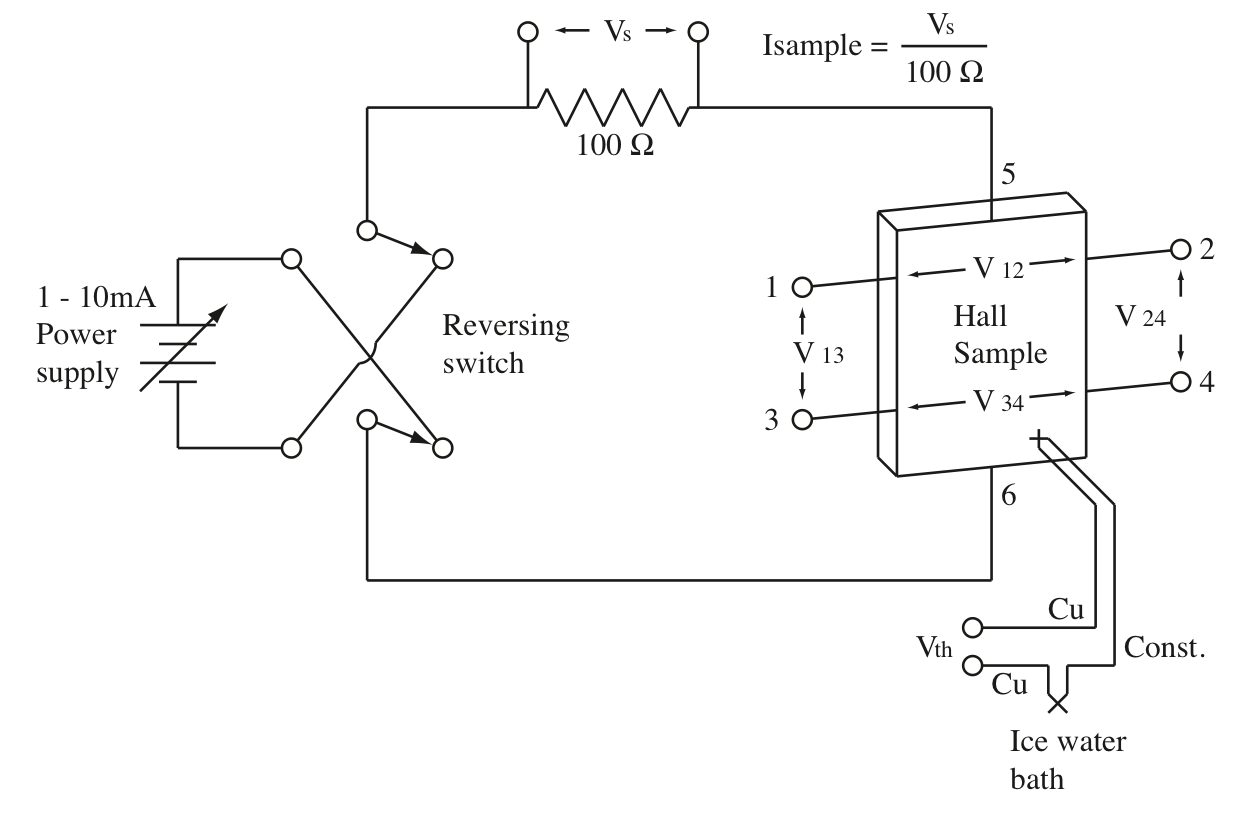
\includegraphics[width=\linewidth]{circuit_diagram.png}
        \caption{A wiring diagram for our experimental apparatus - this is illustrative in understanding the mechanics of the data collection process.~\label{circuit_diagram}~\cite{lab_manual}}
      \end{figure}

      \begin{figure}[h]
        \centering
        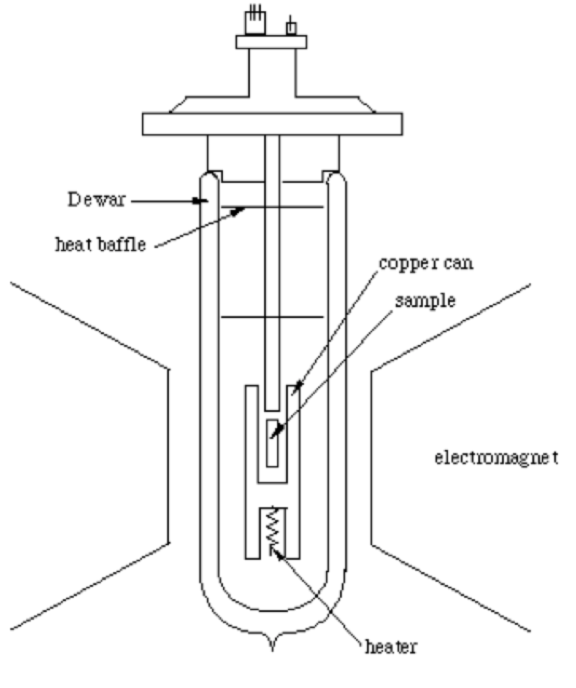
\includegraphics[width=\linewidth]{dewar.png}
        \caption{This shows the cryostat that held our GeGa sample.  The inside, as we can see, was glass to avoid heat conduction to the outer walls of the dewar.  The whole ensemble was placed between the poles of an electromagnet used to produce the strong $\vec{B}$ field that we needed in order to make measurements of our sample.  The whole apparatus turned through an angle of $2\pi$, with detents at $0$ and $\pi$ so that we could accurately take data at two rotations differing by exactly $\pi$.~\label{dewar}~\cite{lab_manual}}
      \end{figure}

      \begin{figure}[h]
        \centering
        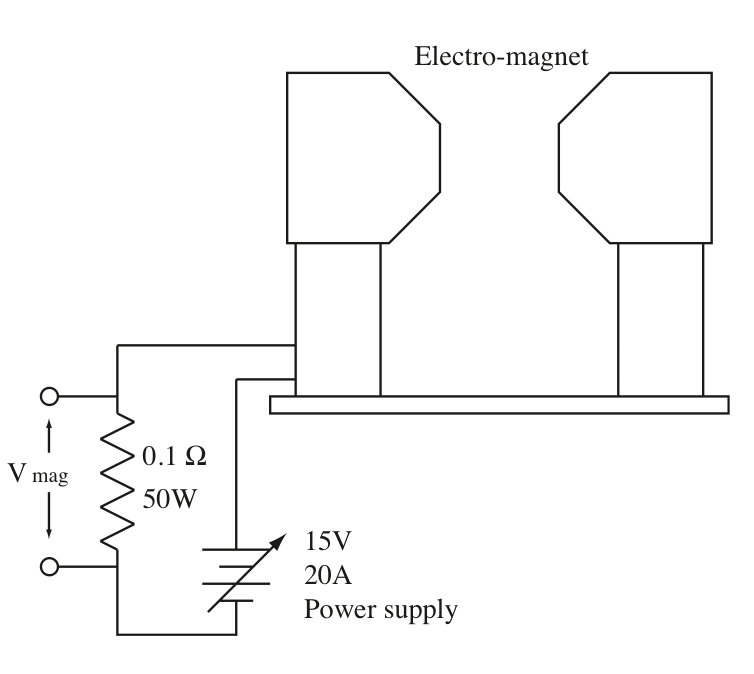
\includegraphics[width=\linewidth]{magnet_setup.png}
        \caption{We needed an extraordinarily strong magnet to see the Hall effect in action, thus we have a large solenoid with an iron core that directs the field generated by the 1000-turn electromagnet through the sample to achieve a field of $900\pm50$ Gauss at the center of the apparatus.~\label{magnet}~\cite{lab_manual}}
      \end{figure}

    \end{widetext}

  \bibliography{bibliography}
  \bibliographystyle{plain}

\end{document}
